\chapter{Marco Experimental}
En este capítulo se describirán los dataset utilizados en el estudio, además de las medidas usadas para valorar los resultados y los parámetros de la red neuronal usadas para predicción.\newline

\section{Datasets}
Los datasets utilizados para el desarrollo de este estudio son:\newline
\begin{itemize}
	\item \textbf{Adiac}. El dataset Adiac contiene los datos de un estudio sobre algas unicelulares basados en imágenes, para pasarla a series temporales se usó el contorno de cada una de las algas en las imágenes. El dataset contiene 390 instancias para entrenamiento y 391 instancias para test, cada uno de los datos cuenta con 176 características y hay 37 clases diferentes. El objetivo es aprender a diferenciar correctamente cada una de las algas.
	\item \textbf{Swedish Leaf}. El dataset Swedish Leaf se trata de un conjunto de datos que contiene el contorno de hojas de árboles suecos. Este conjunto de datos contiene 500 imágenes para entrenamiento, 625 para test, 128 características y 15 clases distintas. El objetivo es aprender a diferenciar cada una de las hojas según su silueta.
	\item \textbf{EGG eye}. La información en este dataset fue obtenida con una medición EGG (medición de actividad eléctrica en el cerebro durante un tiempo)  mediante un sensor. El objetivo de este dataset es diferenciar entre un ojo cerrado y otro abierto. El dataset contiene 14980 instancias y 15 atributos.
	\item \textbf{Face All}. El dataset contiene el contorno de 14 personas diferentes; el conjunto de entrenamiento cuenta con 560 imágenes y el conjunto de test con 1690. El objetivo es diferenciar la silueta de cada una de las personas.
	\item \textbf{Ozone}. Este dataset contiene 2536 instancias, cada una con de ellas con 73 atributos. El objetivo de este dataset es diferenciar entre un día normal y un día con niveles extraños de ozono, para ello se utilizan información de sensores sobre velocidad del viento, temperatura máxima, etc… Este conjunto de datos contiene un gran desbalanceo entre ambas clases.
	\item \textbf{HAR}. El dataset HAR contiene información sobre el movimiento de personas utilizando diferentes sensores en un móvil (giróscopo, acelerómetro, etc…). El objetivo de este dataset es diferenciar entre 6 actividades diferentes. Cada una de las instancias de este dataset contiene 561 características.
	\item \textbf{Wafer}. Este dataset contiene 2 clases, tiene 1000 datos para entrenamiento y 6164 para test; cada uno de los datos contiene 152 características. Los datos de este dataset contiene los valores de datos obtenidos por sensores (cada una de las columnas) para un proceso de creación de planchas de semiconductores para procesadores. El objetivo es distinguir entre planchas defectuosas y no defectuosas. El conjunto de datos contiene un gran desbalanceo entre clases.
	\item \textbf{Yoga}. El dataset contiene 2 clases, tiene 300 datos para entrenamiento y 3000 para test; cada uno de los datos contiene 426 características.El objetivo en este dataset es diferenciar entre una mujer y hombre realizando yoga en imágenes. Los datos que contienen este dataset transformaciones de una imagen a una señal unidimensional, para ello tomaron el outline de cada imagen y se mide la distancia de cada punto con el centro.
\end{itemize}
\verticalspace

Como se ha podido ver en la descripción, algunos de los conjuntos de datos son multiclase, por ello, dichos dataset se han transformado a problemas binarios escogiendo una clase, haciendo esa clase positiva y estableciendo el resto de clases como negativa; de esta forma también se crea desbalanceo entre clases.\newline

\section{Medidas utilizadas}
En este apartado se describirán las medidas utilizadas en el estudio, así como las características de cada una de ellas.\newline

Como ya se mencionó en el segundo capítulo, las medidas usuales no sirven para problemas con desbalanceo, por ello hay que utilizar diferentes medidas que sean útiles para este tipo de problemas.\newline

Antes de describir las diferentes medidas que se van a utilizar, se van a describir algunos conceptos básicos sobre problemas de clasificación. Un modelo de clasificación o clasificador es una función que permite decidir qué elementos de un conjunto de datos pertenecen a una cierta clase; para realizar esta decisión, el clasificador puede utilizar un umbral sobre un valor real o directamente obtener un valor discreto.\newline

Pongamos el caso de un problema de clasificación binario, en la que los datos se clasifican como positivos, lo representaremos con la letra p, o negativos, lo representaremos con la letra n. Una vez se ha entrenado un clasificador y se han obtenido los resultados, estos se pueden representar en una Matriz de confusión (para clasificación binaria es una matriz de 2x2) de la siguiente forma.\newline

\begin{figure}[h]
	\centering
	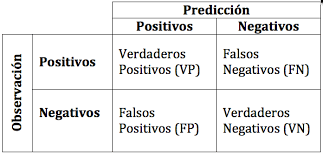
\includegraphics[width=90mm]{imagenes/conf-matrix.png}
	\label{fig:61}
	\caption{Ejemplo matriz de confusión.}
\end{figure}

Los Verdaderos Positivos (VP) son aquellos datos que han sido clasificados como positivo y su clase real es positiva, los Verdaderos Negativos (VN) son aquellos datos que han sido clasificados como negativos y su clase real es negativa, los Falsos Negativos (FN) son aquellos datos que han sido clasificados como negativos y su clase real es positiva; por último, los Falsos Positivos (FP) son aquellos datos que han sido clasificados como positivos pero su clase real es negativa.\newline

Sabiendo los valores de cada uno de estos datos, se pueden calcular medidas que contemplen un mal rendimiento por parte del clasificador al predecir alguna de las clases; esto es interesante para problemas con desbalanceo porque permite ver el rendimiento específico del clasificador para predecir la clase minoritaria.\newline

Las medidas que se utilizarán para el estudio son las siguientes: AUC, Precision, Recall, F1 Score y G-Mean.\newline

La medida Precision representa el porcentaje de los datos clasificados como positivos que realmente son positivos, es decir, de todos los datos que el clasificador ha predicho como positivos, cuántos de ellos son realmente positivos. Esta medida toma valores entre 0 y 1, valores cercanos a 1 indican un buen rendimiento por el clasificador para reconocer datos de la clase positiva. Esta medida se representa como:\newline
$$ Precision = \frac{TP}{TP + FP} $$

La medida de Recall o también conocida como True Positive Rate (TPR) representa el número el porcentaje de datos de la clase positiva que han sido clasificados como positivos. Toma valores entre 0 y 1, valores cercanos a 1 indican un buen rendimiento para reconocer la clase positiva, si el clasificador no fuera capaz de reconocer la clase positiva el número de Falsos Negativos sería muy alto y su valor se acercaría a 0.Esta medida se puede expresar como:\newline
$$ Recall = \frac{TP}{TP + FN} $$


A su vez, existe la medida True Negative Rate (TNR), que representa el porcentaje de ejemplos negativos bien clasificados, se define con la siguiente expresión.\newline
$$ TNR = \frac{TN}{TN + FP} $$

La medida F1 Score tiene en cuenta las dos anteriores para ser calculada, puede expresarse como:\newline
$$ F_1 Score = 2 * \frac{Precision*Recall}{Precision+Recall} $$

Esta medida mide el equilibrio entre las medidas Precision y Recall, si alguna de las dos tiene un valor bajo, el valor de F1 Score baja, para que aumente, el valor de ambas medidas debe aumentar. Toma valores entre 0 y 1.\newline

La medida G-Mean representa la media geométrica, sirve también para medir el equilibrio entre Precision y Recall. Se representa de la siguiente forma:\newline
$$ G-Mean = \sqrt{Precision*Recall} $$

Para esta medida, si cualquier de las medidas toma valores bajo su valor es 0.\newline
La última medida es AUC (Area Under Curve), esta medida representa el área bajo la curva ROC. La curva ROC es una representación gráfica del rendimiento entre TPR y TNR; cuanto más alto sea el valor de ambas medidas, mayor será el valor de la medida AUC.\newline

\begin{figure}[h]
	\centering
	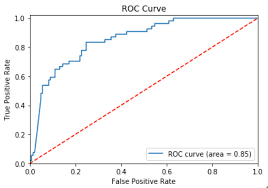
\includegraphics[width=90mm]{imagenes/auc.png}
	\label{fig:62}
	\caption{Ejemplo curva ROC.}
\end{figure}
\verticalspace

A partir de esta medida se puede medir el rendimiento de un clasificador, si el valor de AUC es 1, entonces el clasificador es perfecto. Si un clasificador hiciera las predicciones de forma aleatoria, su valor de AUC sería 0.5 y por lo tanto cualquier clasificador con valores cercanos o por debajo se considera que el clasificador es malo; para valores a partir de 0.7-0.75 se puede decir que el clasificador es aceptable.

\section{Parámetros de la red}
En este apartado se va a describir la estructura de la red utilizada en este estudio.\newline

Como se comentó anteriormente, la red usada está formada por un conjunto de LSTMs para procesar la información de las series temporales.\newline

La red básica utilizada está formada por dos capas; una capa formada por 32 LSTM y otra formada por una única neurona conectada a todas las LSTM usada para calcular la clase; para ello utiliza una función sigmoide como salida de la neurona. La estructura tendría la siguiente forma.\newline

\begin{figure}[h]
	\centering
	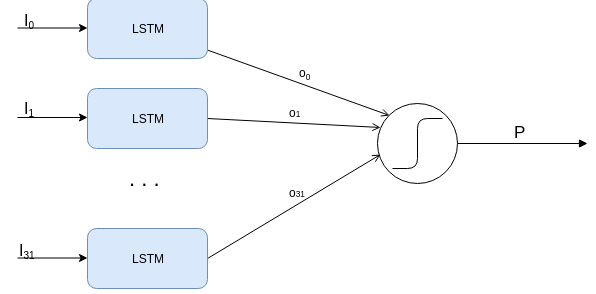
\includegraphics[width=100mm]{imagenes/Estructura_Red.png}
	\label{fig:63}
\end{figure}
\verticalspace
Cuando se define la capa de LSTM, se debe especificar el tamaño de la entrada que tendrá la LSTM; como en el caso de este estudio se utilizan diferentes tamaños de ventana, el tamaño de la entrada para la LSTM se especifica como $(1, tamventana * nseries )$, de esta forma cada LSTM procesa una ventana de información en cada momento.\newline

Por último, la red utiliza 50 epochs para entrenar y un tamaño para el batch de 16.